
\section{Selecting Platforms in CLIC}

A logical plan needs to be transformed into a physical plan before being actually executed.
That is, selecting each logical operator a physical platform to transform to the physical operator.
However, assuming that a logical plan has N operators, and each operator has K available physical platforms to choose from, 
there exist $K^N$ available combinations.
Even so, there is still a best platform for each operator, on which deploying the operator can achieve the best overall performance. 
We take the best platform as the label of this operator.
The label of one operator is not fixed, but change by multiple factors.
Therefore, the goal of the platform selection is CLIC is to find this label for each logical operator in a logical plan to achieve the best overall performance.


In CLIC, a logical plan is organized in the form of DAG where the node denotes the logical operator and the edge denotes the operator dependency.
Selecting the label of each node in a graph is actually a typical node classification problem.
Such problems with topology as input are usually solved with the Graph Neural Network(GNN) because it can be directly applied to the graph structure without encoding it to a vector first[].
Among many GNNs, GCN is considered better at solving the node classification problem because of its ability of capturing neighbor relationships with its convolution kernel[].
Compared with the ML-based a pproach, GCN avoids the loss of structural information due to the need of encoding the topological structure as a vector[];
One more step before feeding the logical plan into GCN is to vectorize the operator, i.e transform the operator object into a numerical vector.
However, as we have disscussed in Section 2.2, the traditional vectorization method is not suitable for CLIC. 
% those drawbacks ? 第二章要不要说呢?说了的话这能直接用 the、those 吗?
Inspired by the word embedding[], we propose the operator embedding and overcome those drawbacks for the first time.
In 5.1, we give a first look to the the naive encoding approach and discuss its limitations, and then we introduce our embedding-based encoding.
In 5.2, we detailed the process of using GCN to select platforms through an example.
In 5.3, we introduce the method of synthesizing training data of the operator embedding and the GCN.

\subsection{Feature Extraction}
As it turns out, many Machine Learning algorithms and almost all Deep Learning Architectures are incapable of processing raw form data like plain text or, in this case, the operator object. 
They require numbers as inputs to perform jobs like classification, regression etc. in broad terms. 
Therefore, the operator needs to be encoded as the numerical vector before fed into GCN.

When designing the feature vector, we consider the following three most influential factors: the operator itself, hardware, and workload.

\subsubsection{Operator Encoding}
Operators describe the computation logic of the workflow.
Two logical plans with the same topology can express different computation because of the consisted operators.
As examplified in Figure \ref{fig:graph-comparison}, although both of the red and the blue plans have the same topology,
the red one consists of relational operators and expresses a SQL query, while the blue one consists of linear operators and expresses a mathmatical calculation.
As a result, they need to be classified to the different execution engines, such as Postgre for the former and Tensorflow for the latter.

\begin{figure}
  \centering
  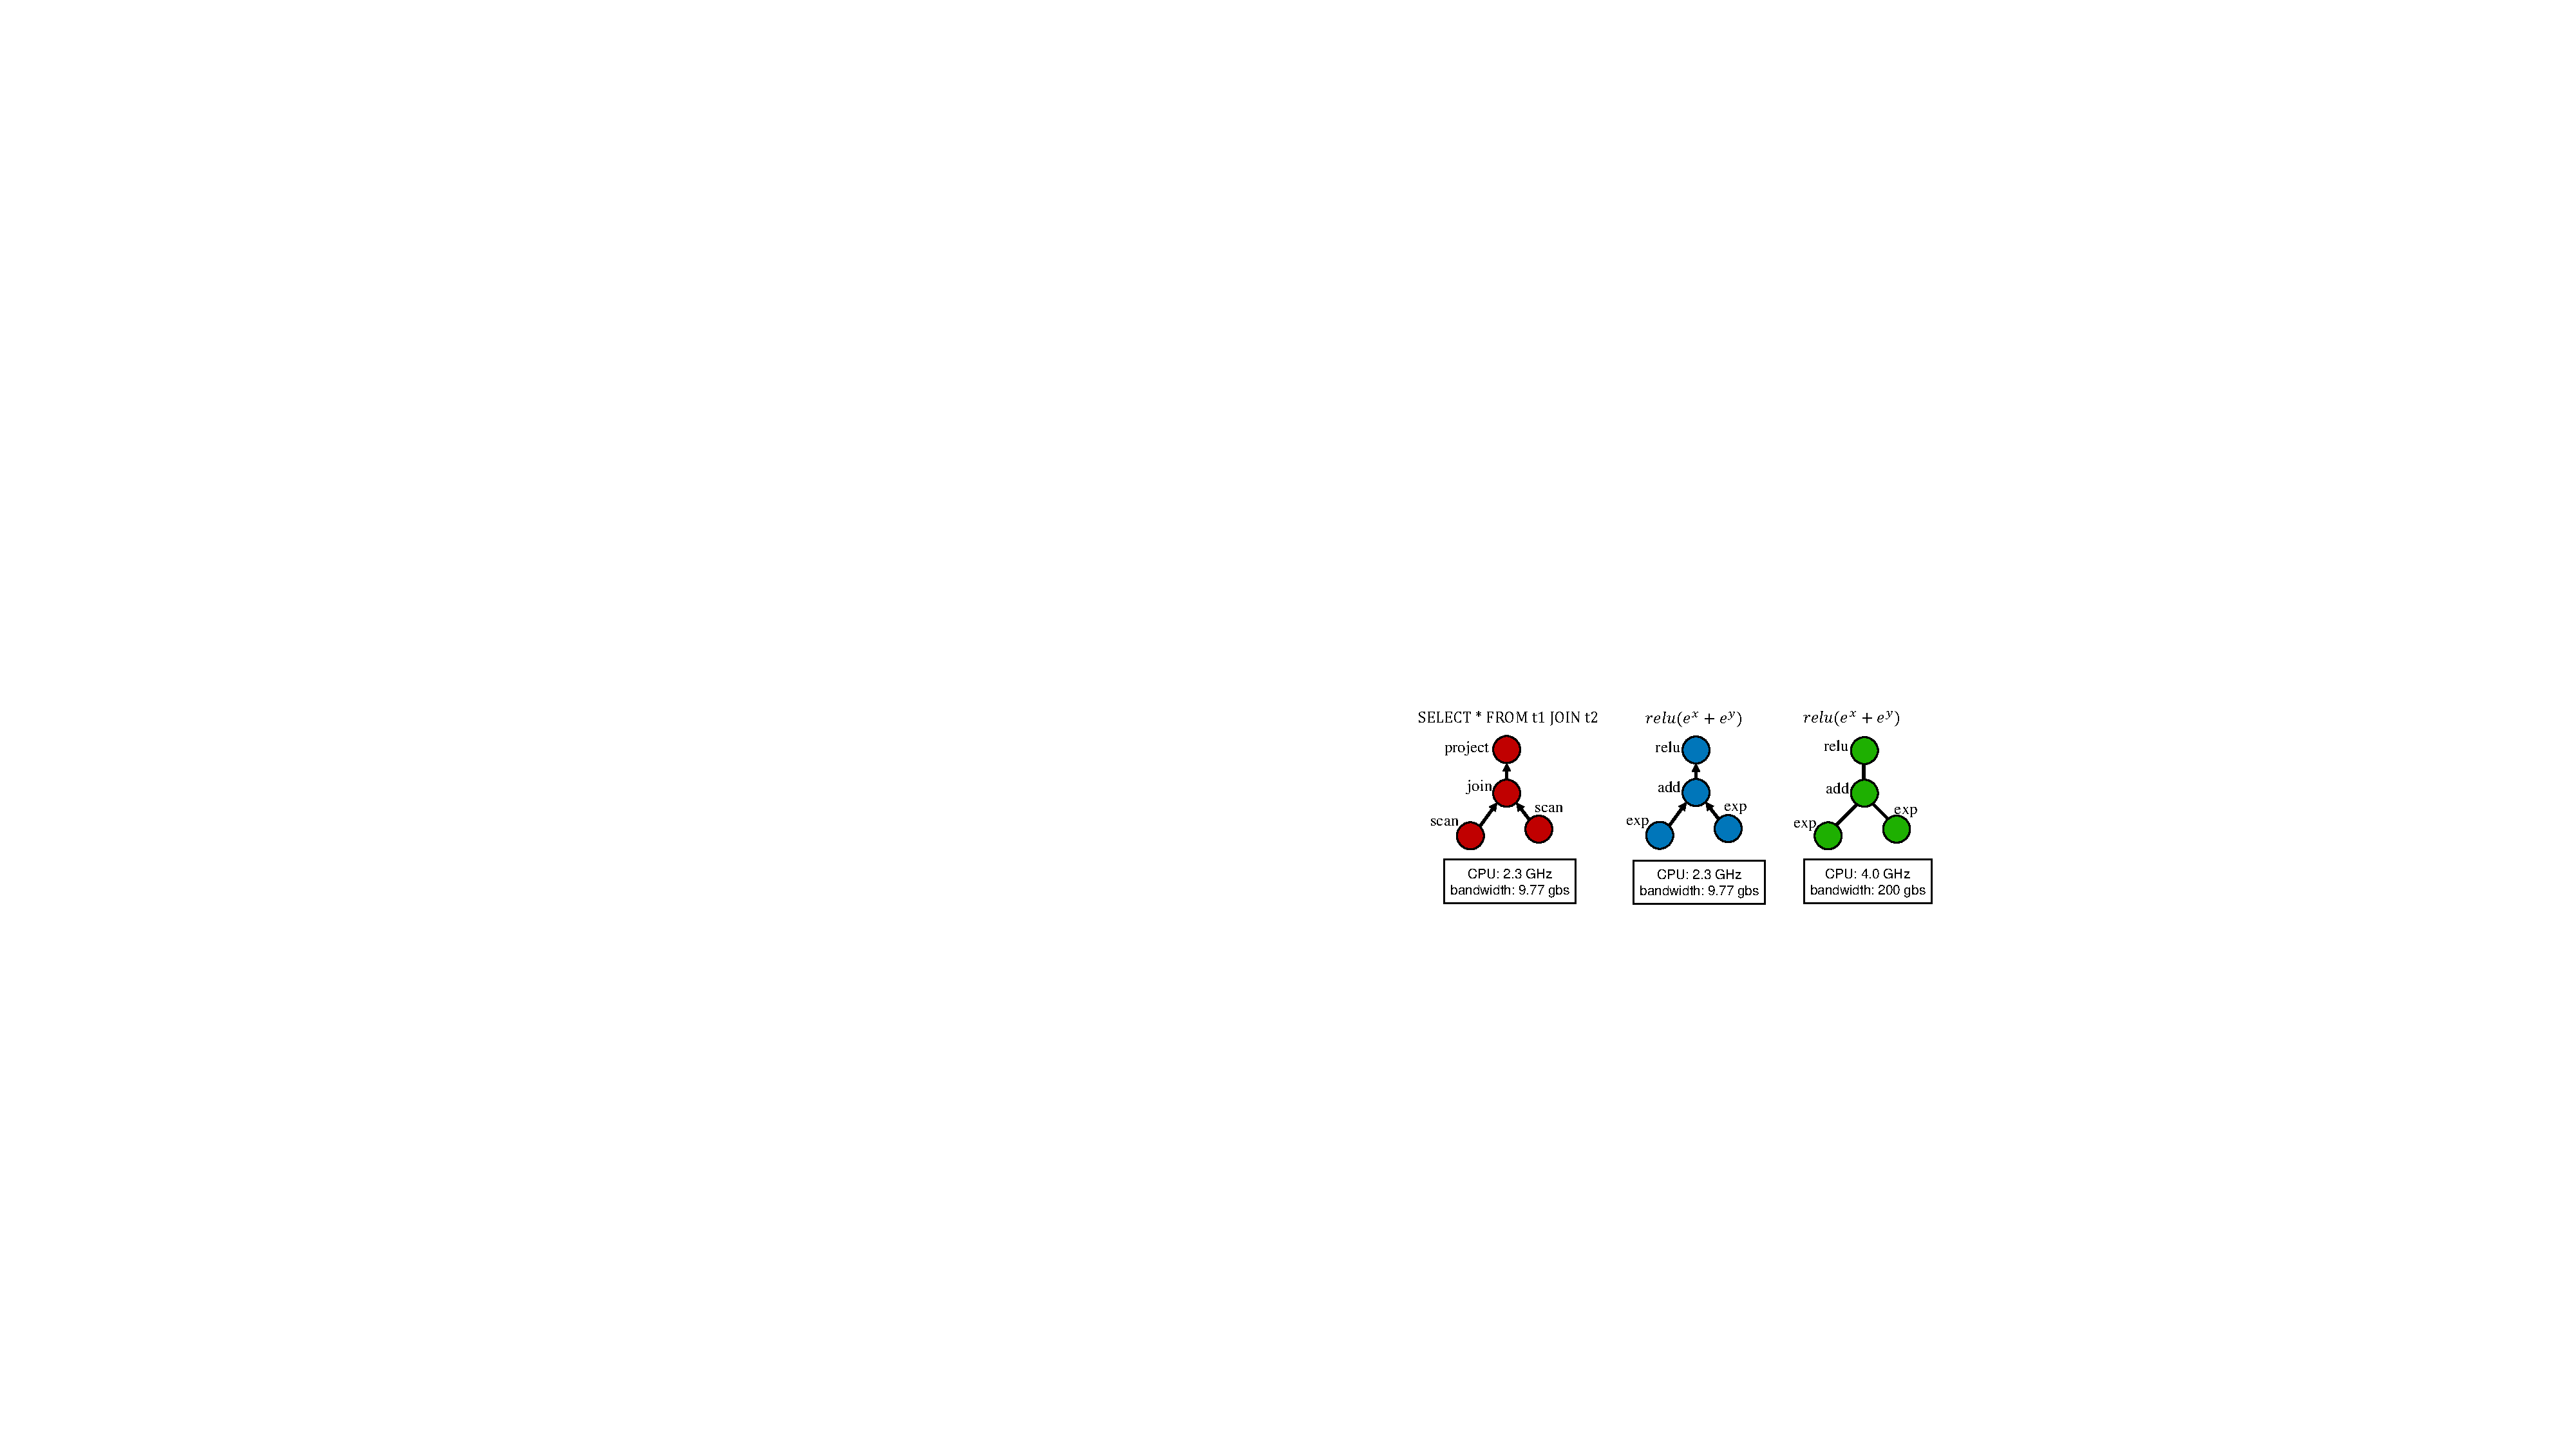
\includegraphics[width=0.7\linewidth]{figures/graph-comparison.pdf}
  \caption{Plans with the same topology}
  \label{fig:graph-comparison}
\end{figure}

We first follow the traditional approach that using the one-hot encoding to represent the operators.

\textbf{One-Hot Encoding}
One-hot encoding is an simple but effective vectorization method that has been widely adopted in vectorizing the category features, such as gender or id. 
The vectorization result is a 0-1 vector whose dimension is equal to the number of categories.
The blue segment of the feature vector in Figure \ref{fig:feature-vector-onehot} illustrates the one-hot encoding. 
As we can see that, each row stands for an operator and only has one non-zero element at its corresponding column.

\begin{figure}
  \subfigure[One-Hot Encoding]{
      \label{fig:feature-vector-onehot}
      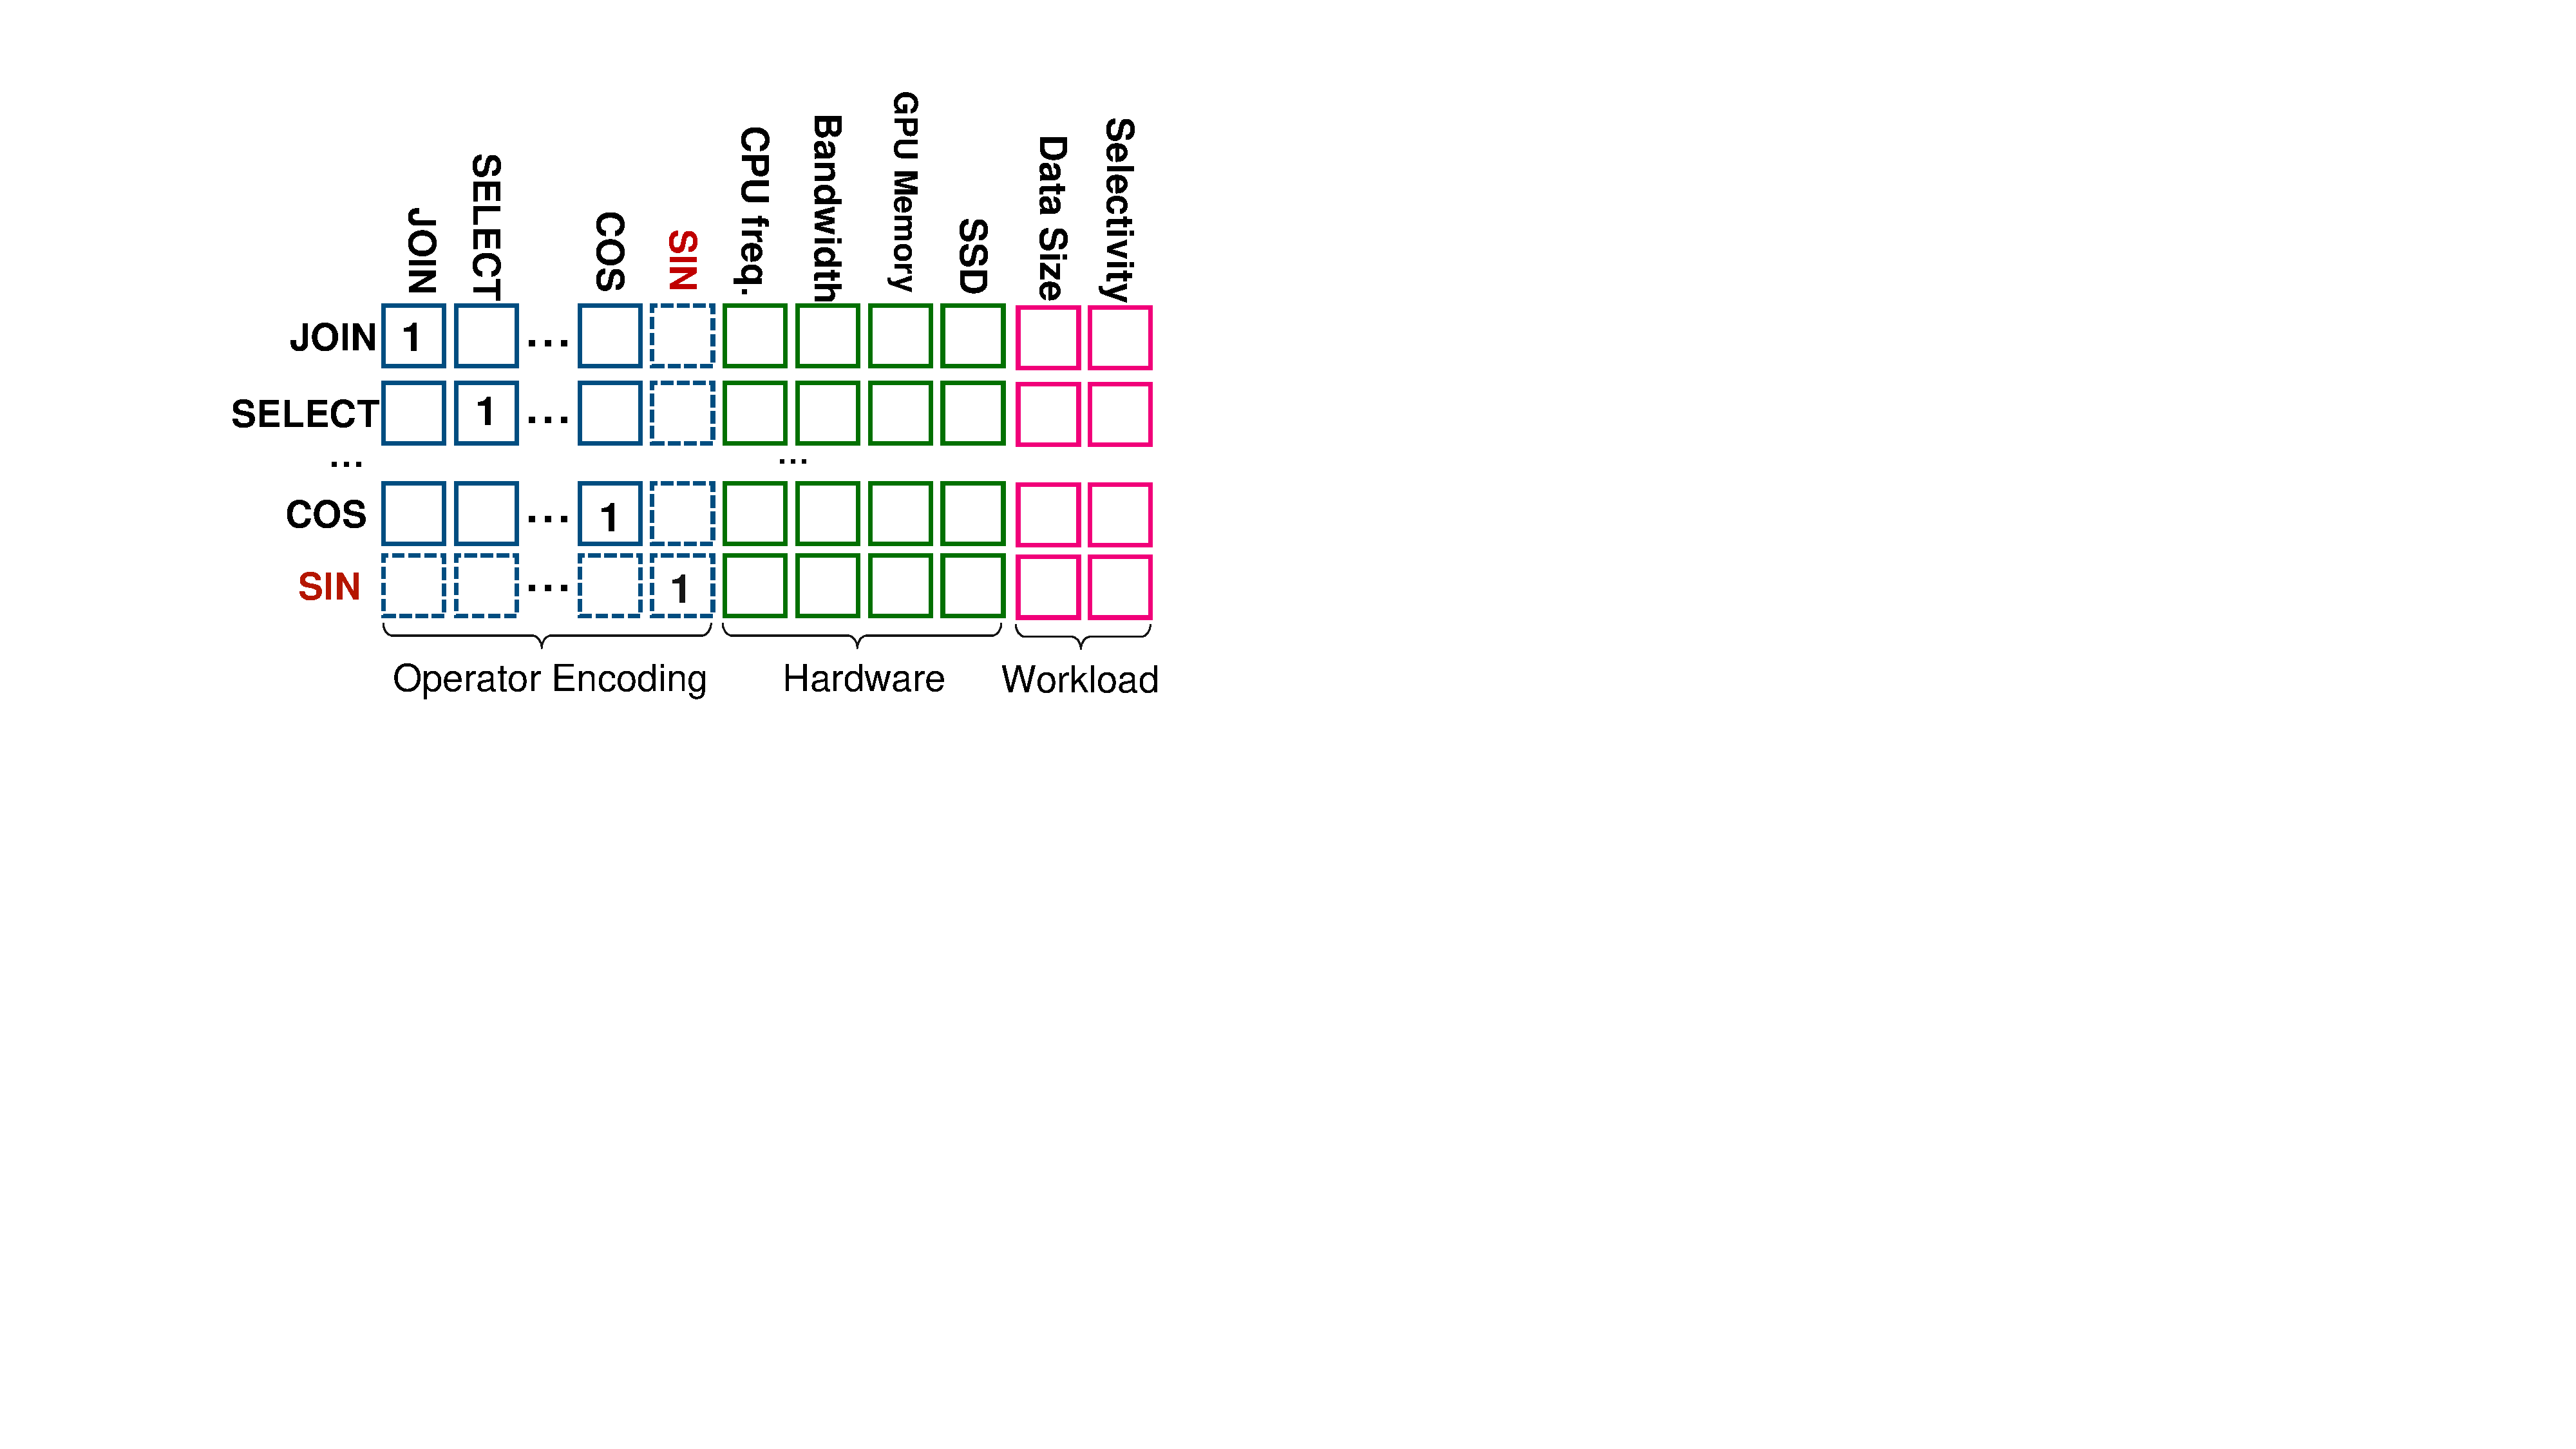
\includegraphics[width=0.47\linewidth]{figures/feature-vector-onehot.pdf}
  } 
  \subfigure[Operator Embedding]{
      \label{fig:feature-vector-embedding}
      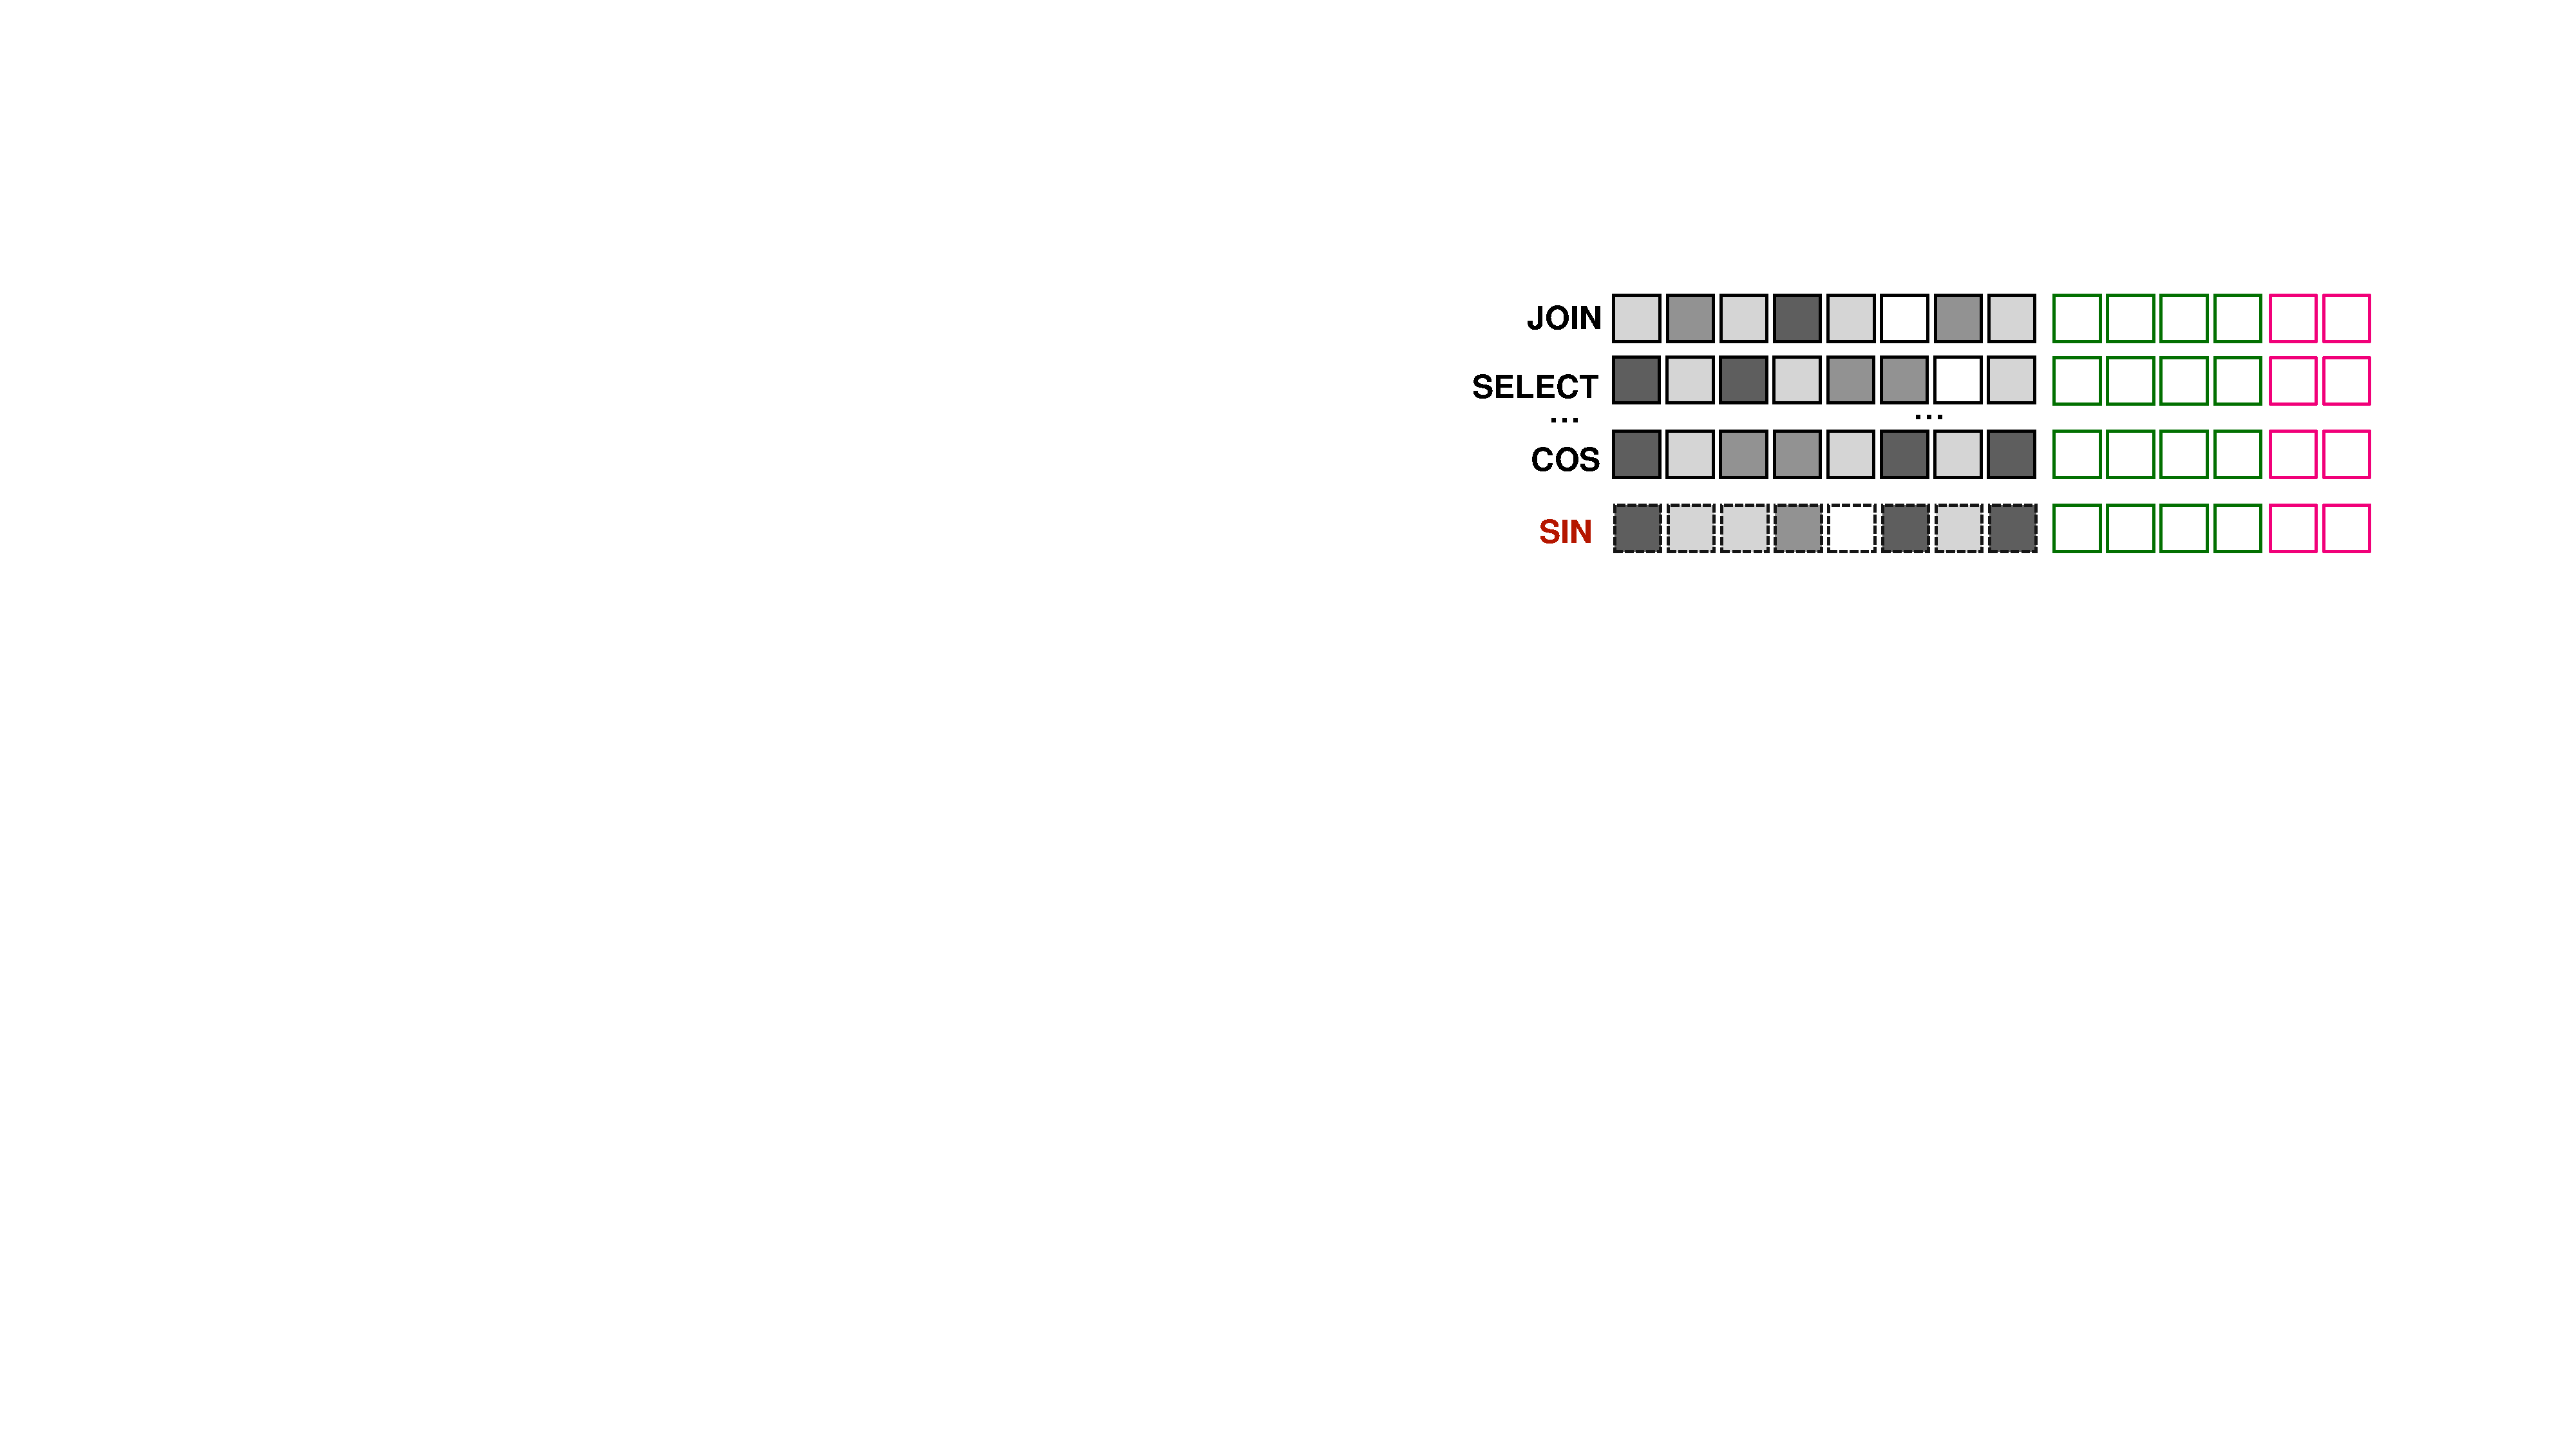
\includegraphics[width=0.47  \linewidth]{figures/feature-vector-embedding.pdf}
  } 
  \caption{Feature Vector Comparison}
  \label{fig:feature-vector}
\end{figure}

However, this encoding has two prominent limitations that are especially obvious in CLIC:

1) Low computational: 
The dimension of the one-hot encoding is equal to the category amounts and the vector has only one non-zero element.
Therefore, as the number of categories grow up, the one-hot encoding usually resulting in a high-dimensional and sparse vector. 
Generally speaking, this makes it less computational since the majority of neural network toolkits do not play well with very high-dimensional, sparse vectors [Neural Network Methods in Natural Language Processing, 2017]. 
Since a cross-platform framework like CLIC usually need to train a cost model but face the insufficient training data problem, 
this limitation becomes more crucial to them.

2) Imcompatible to a new operator integration: 
In particular, as a new operator been integrated, the dimension of the one-hot vector will grow in the same time. 
Figure \ref{fig:feature-vector-onehot} examplified this situation. 
When the new \textit{SIN} operator (the red operator) being inserted, all the vectors' dimensions are grown by one (represented by dash line).
The consequnce is that the pre-trained model, GCN for example, needs to be retrained because the higher dimension conflicts with the model's input requirement.
This problem does not exist in most scenarios, because the dimensions of the input data are usually predefined and will not grow.
However, as we have narrated in Section 2, a cross-platform system experiences fast evolutions, such as enriching the operator library.
Under this circumstance, the dimension of the one-hot vector will vary frequently, which further lead to the frequent model retraining.


In order to overcome the above two limitations, we propose our operator embedding.
% 为了克服以上两个问题,我们提出了新的使用运算符嵌入(operator embedding)向量化运算符的方式。

\textbf{Operator Embedding}
In mathmatic, an embedding is a function $f(X) -> Y$ that maps a data point X in one space to point Y in another space[wiki]. 
This is the most important preprocessing technique in natural language processing (NLP), where the word embedding is used for the representation of words for text analysis. 
It is typically in the form of a real-valued vector that encodes the meaning of the word such that the words that are closer (cosine distance) in the vector space are expected to be similar in meaning [wiki]. 
For promotion, there also are image embedding, video embedding. 
A representative algorithm for generating word embedding is the CBOW[], whose idea is that words appearing in the same sentence have higher relevance. 
The way CBOW works, in a nutshell, is that it tends to maximize the joint probability of a word and its context words in a sentence. 
Generating the word embedding using CBOW requires a large corpus containing enough sentences as the training dateset to learn the word relationships.

Back to CLIC, we reasonably assume that operators also have semantical meanings and are relevant to the others in the same logical plan.
The semantical meanings, for example, include operator's computing paradigm, \#input/output, etc.
Based on these assumptions, we design the operator embedding.

As illustrated in Figure \ref{fig:feature-vector-embedding}, 
the operator embedding is a real-valued continuous vector whose dimension is fixed (hyper parameter) and usually rather smaller than that of the one-hot encoding.
It has two key characteristics that can overcome the above one-hot encoding's limitations:
1) Low-dimensional and Dense. 
Compare to one-hot encoding's high-dimensional 0-1 vector, 
the operator embedding is encoded with real-world meanings and therefore only a low-dimensional vector is required to represent an operator.
This makes it more computational for the following models, and in the meantime, saves a lot of training data.

2) Compatible to the operator evolution. The embedding's dimensions will not grow with the integration of new operators. 
As we can see from Figure \ref{fig:feature-vector-embedding}, the newly integrated \textit{SIN} operator has consistent dimension with the others.
The model that takes it as input data does not need to be retrained anymore. 
This largely supports the fast evolution of CLIC.

To generate the operator embedding, we share the same ideas in the word embedding that
1) allowing semantically similar operators to have closer (cosine) distance, 
and 2) maximizing the joint probability of an operator and its neighbour operators in a logical plan.
Therefore, we can still adopt the CBOW algorithm.
We consider the topological ordered logical plan as the "sentence", where each operator is a "word" and its neighbors are the "context words". 
The corpus, i.e. logical plan dataset, are retreived from our synthesized dataset which will be discussed later in Section xx.
Using this corpus as dataset, we finally have the trained operator embeddings visualized in Figure \ref{fig:emb_visual}.
We reduce the dimension to the top-2 dimensions with the highest eigenvalue for the sake of visualization.
The observation is that the operator \textit{sin} is closer to \textit{tan} and far from \textit{union}.
This can be explained semantically as that \textit{sin} and \textit{tan} belong to the same computing paradigm and have the same \#inputs/outputs.
Although the meanings of the embedding are more complex than just paradigm and parameter amounts, 
for CLIC, 
we can simply assume that the operator embedding has successfully portrays the operator.
The power of the embedding will further be revealed when utilizing to train the GCN model, which we will later disscuss in Section xx.

\begin{figure}[ht]
  \centering
  \begin{minipage}[b]{0.4\linewidth}
    \centering
    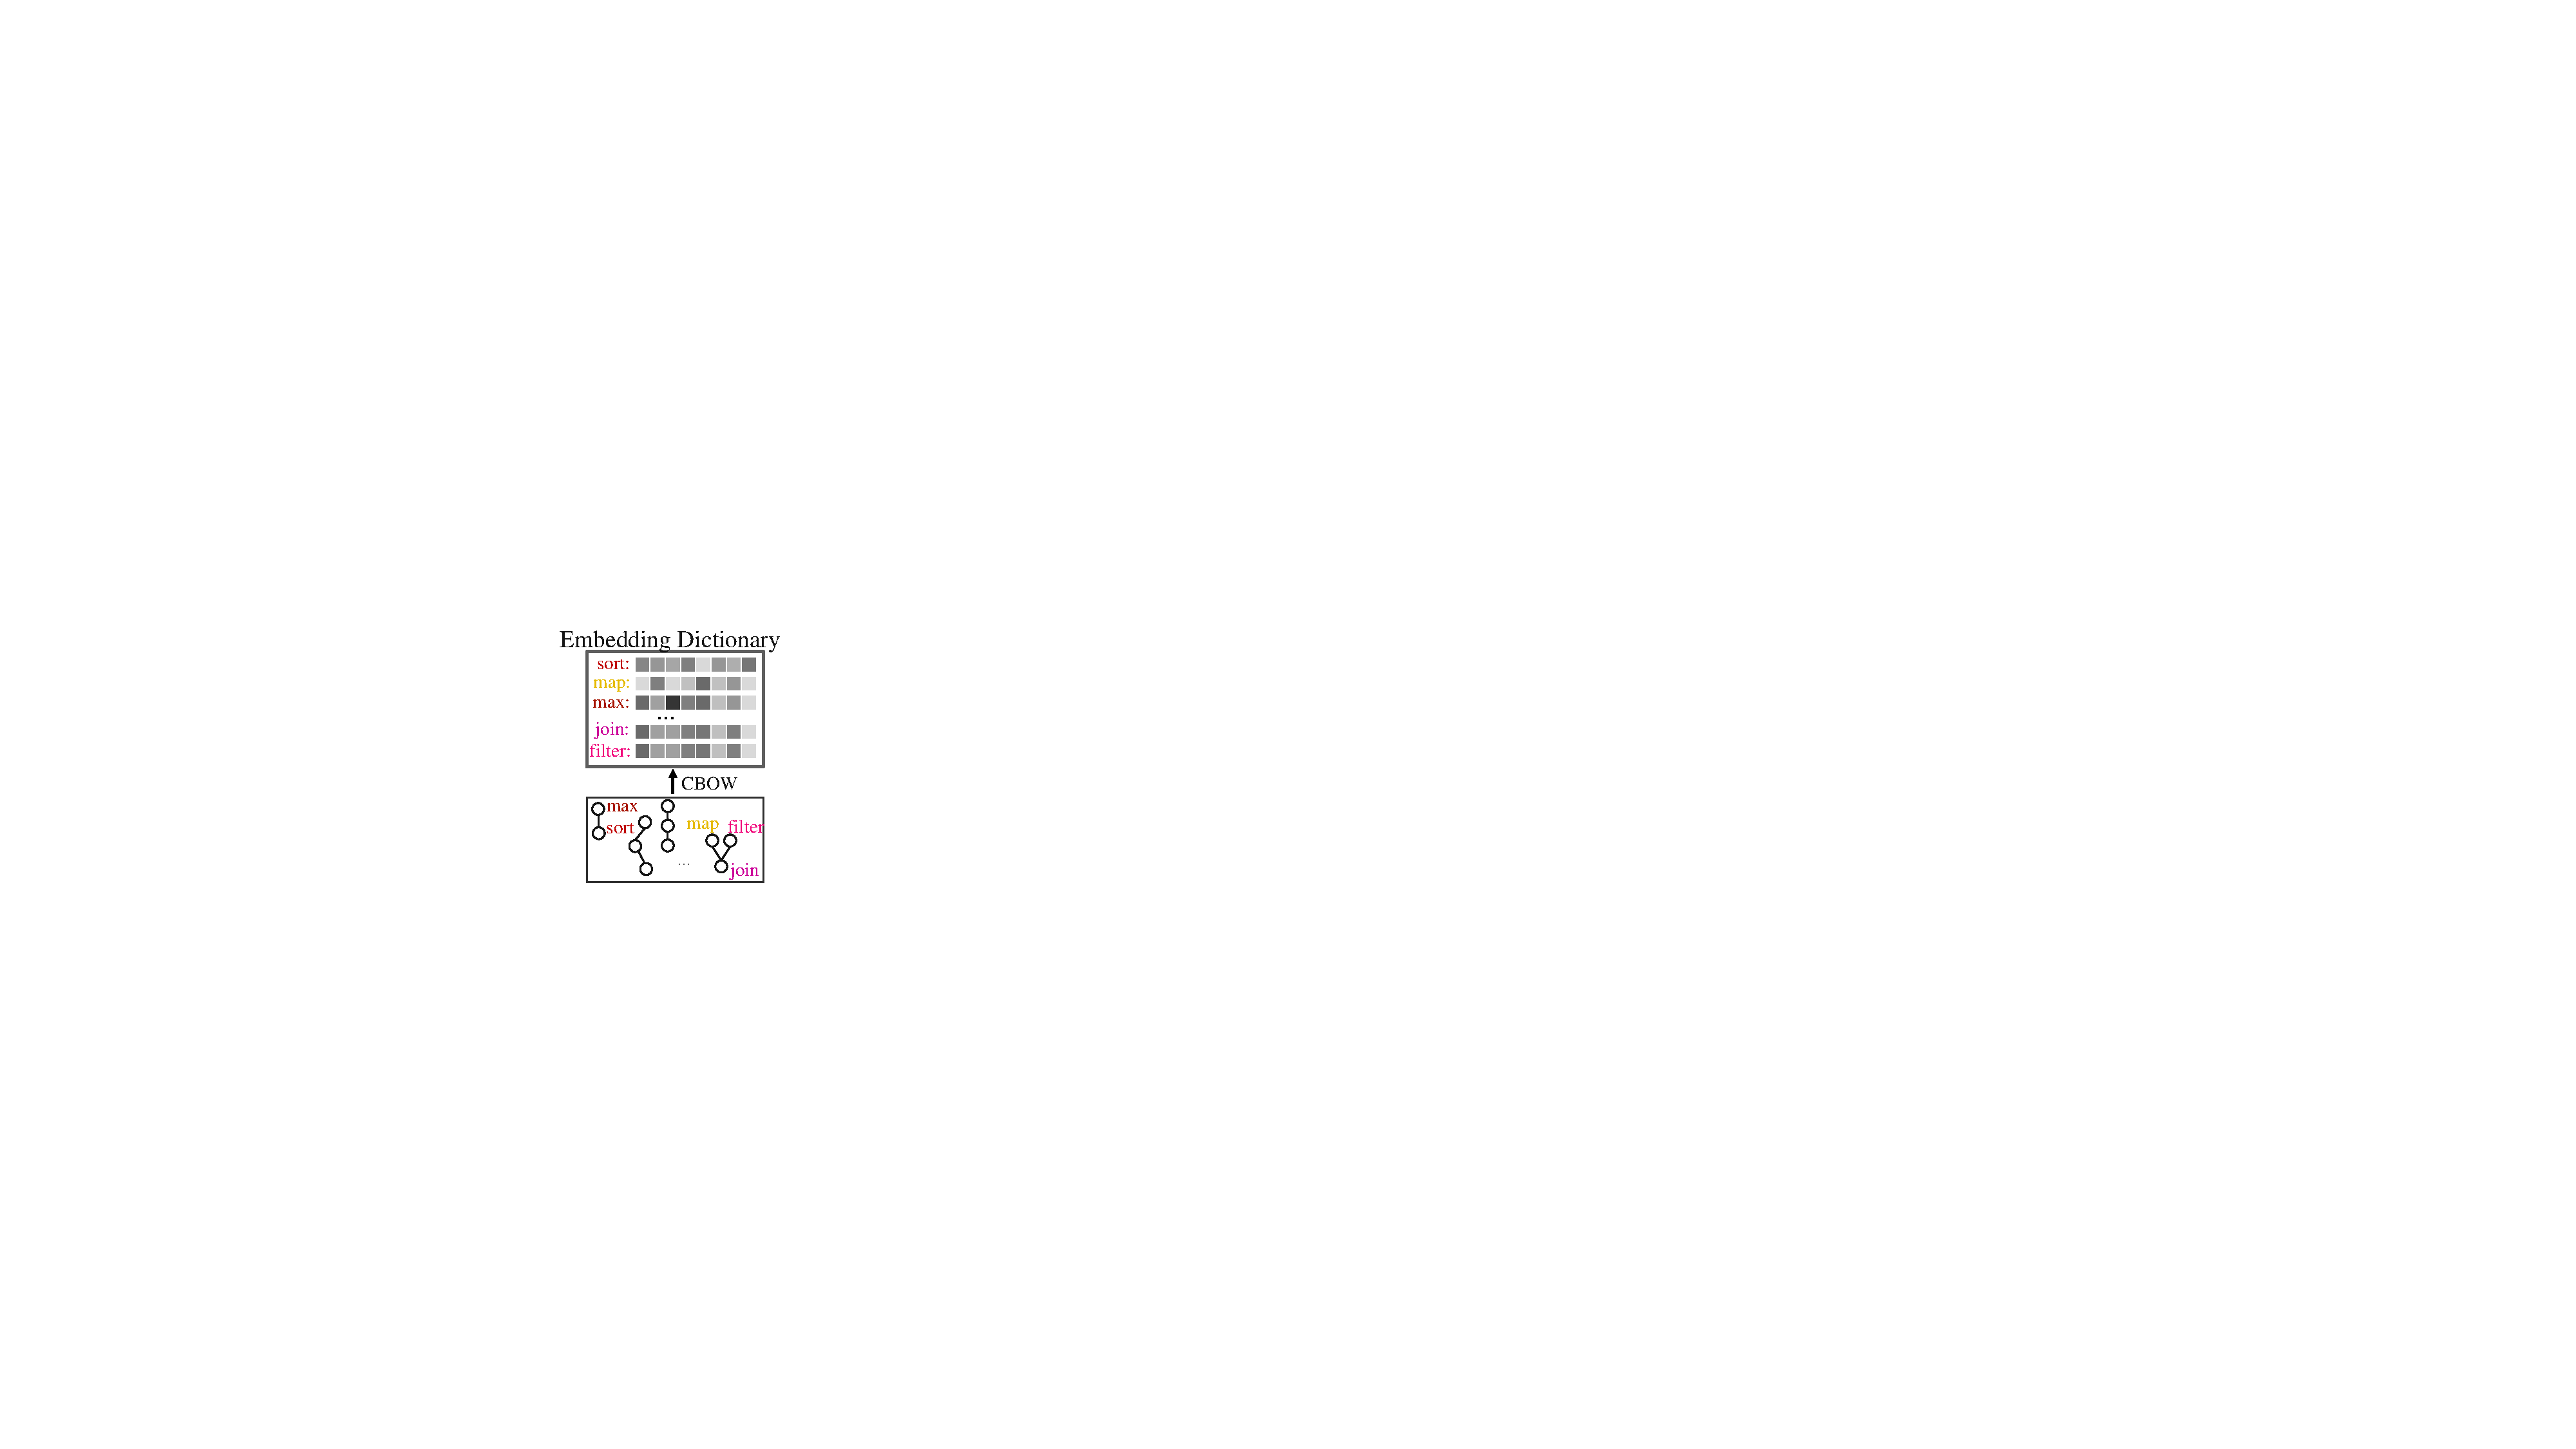
\includegraphics[width=\linewidth]{figures/embedding-training.pdf}
    \caption{Generating Operator Embedding}
    \label{fig:emb_training}
  \end{minipage}
  \quad
  \begin{minipage}[b]{0.55\linewidth}
    \centering
    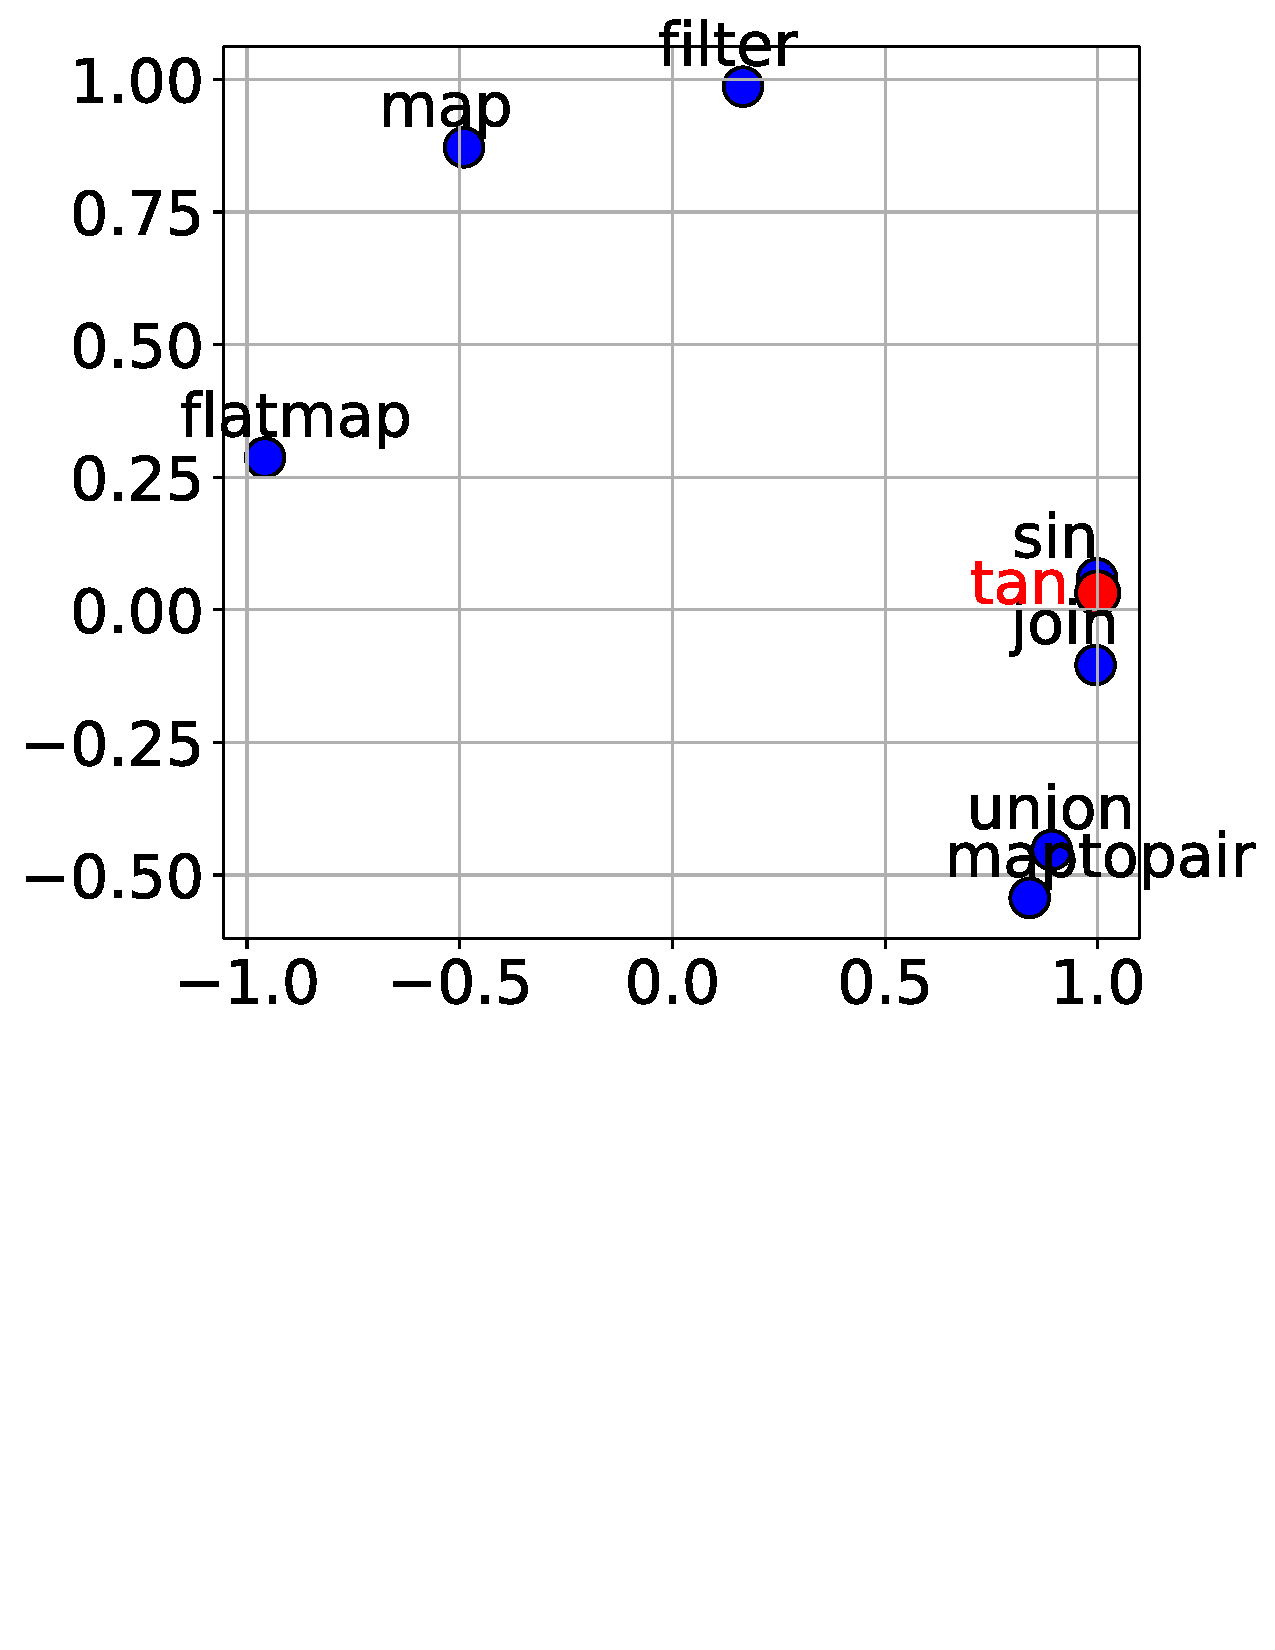
\includegraphics[width=\linewidth]{figures/embedding_visual.pdf}
    \caption{Embedding Visualization}
    \label{fig:emb_visual}
  \end{minipage}
\end{figure}

One thing we want emphasize is that,  
since the operator used as the input of embedding is only logical,
one can generating an operator's embedding whether it is actually implemented by a framework, say CLIC, or not, 
as long as the corpus they offered contains the operator.
In another word, the operator embedding technique is a general encoding method that is independent to any computing frameworks.
What this means to CLIC is that, we can construct a rich operator embedding set as the "dictionary" before we actually implement them.
After that, every time we integrate a new operator, we look up to the dictionary for its embedding. There are two scenario for getting the embedding:

1) The operator is new to CLIC but not the dictionary. In this case, we retreive its embedding directly from the dictionary.

2) The operator is out of the dictionary. In this case, we need to first synthesize some new logical plans that contain this operator according to its attributes (paradigm, \#input/output, etc.), and then re-generating all of the embeddings.


\subsubsection{Hardware}
Hardware resources such as network bandwidth, GPU memory, SSD/HDD, etc. are also important factors affecting platform classification. 
For example, the selection of two different communication model used in ML frameworks, i.e. the parameter server model and the all-reduce model, are effected by the bandwidth and the GPU. 
In general, the parameter server works better if you have a large number of unreliable and not so powerful machine;
All-reduce works better if you have a small amount of fast devices(variance of step time between each device is small) run in a controlled environment with strong connected links. 
The benchmark result in [ML platform Benchmark] and the experiments in Section 2 also support to this. 
Figure \ref{fig:graph-comparison} exhibit the influence of hardware differences that the blue and the green plans are classified to two different platforms, 
say the blue on Tensorflow(parameter-server architecture) and the green for PyTorch(default to all-reduce architecture).
The reason behind is the differences of the cluster configuration, e.g. the node's NIC bandwidth has been upgraded from 9GBS to 200GBS.
Therefore, we also encode some hardware parameters like CPU frequency, bandwidth, etc. into the feature vector, 
as shown in the green segment in Figure \ref{fig:feature-vector}. 
Those fields are the same for all operators in a logical plan. 
For simplicity, we only assume that the nodes in the same cluster all have the same hardware configurations.

\subsubsection{Workload}
% 数据分布和 selectivity
% 还没想好怎么写
% Workload factors include data size, data distribution, selectivity, etc.
nothing here for now.


Put it all together, as shown in Figure \ref{fig:feature-vector-embedding}, 
the final feature vector consists of the operator embedding, hardware, and workload.
Among the three fields, 
the embedding field is different to all operators and is retreived from the pre-generated dictionary; 
the hardware is loaded from the configuration file when CLIC is started and is the same to all operators;
the workload is computed by CLIC during runtime and is the same to all operators.

Next, we are going to introduce how GCN utilizes the feature vector to do node classification.

\subsection{GCN Intuition}

Graph Convolutional Network is a convolutional neural network that can be directly applied to graphs. 
It applies a convolution kernel to learn the first-order spectral feature, which are followed by activation functions to learn graph representations[42]. 
The convolution kernel learns the spectral feature by inspecting neighboring nodes in turn. 
Below we introduce the logical plan's node classification process using GCN, which is shown in Figure \ref{fig:gcn}.

\begin{figure}
  \centering
  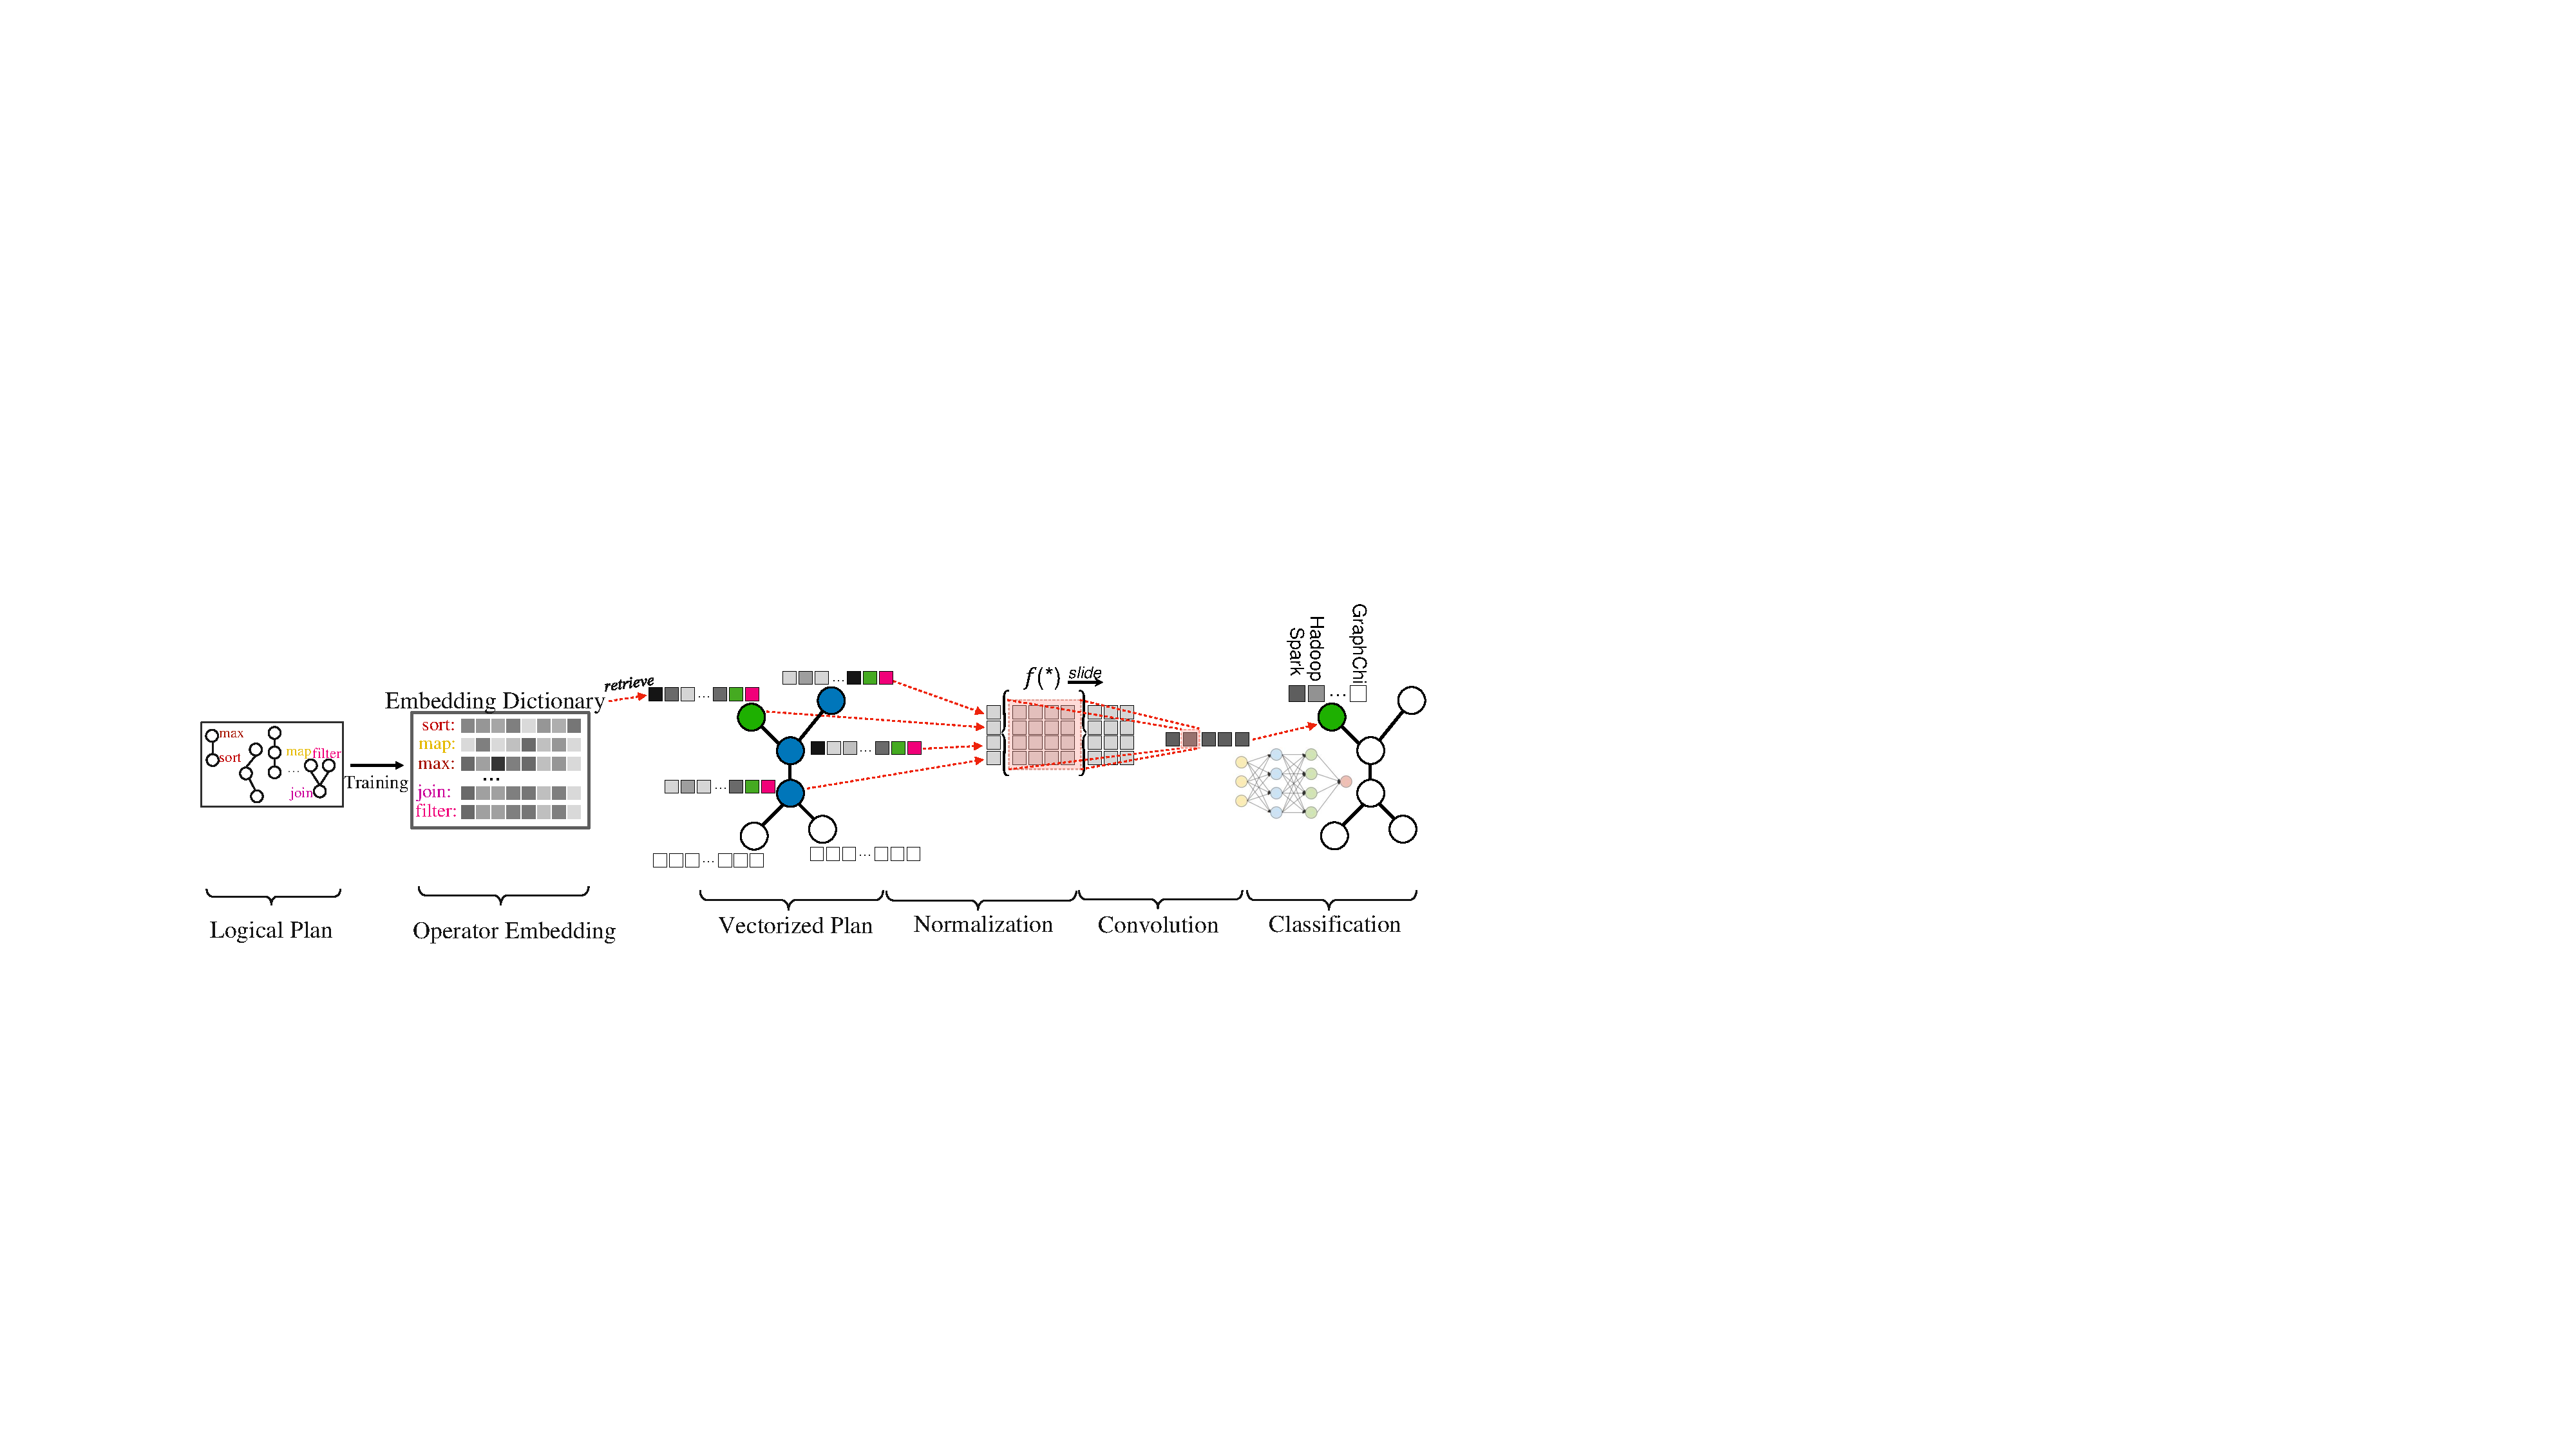
\includegraphics[width=\linewidth]{figures/GCN-new.pdf}
  \caption{Selecting platforms with GCN}
  \label{fig:gcn}
\end{figure}

The input of GCN is a graph with nodes are represented as feature vectors. 
The feature vector, as we have just disscussed, consists with three segments: operator embedding (gray), hardware (green), and workload (pink).
In order to learn the relationship between the current operator (green node) and its neighbors (blue nodes), 
the input topology needs to experience alignment and convolution steps.
The alignment step aligns the irregular topology to the matrix by selecting the current operator and its K-1 (hyper-parameter) neighbors to form the matrix of size $K * |V|$. 
Then during convolution step, the kernel function \footnote{The kernel function takes as input a matrix, 
then dot products it with another pre-defined matrix, 
and finally aggregates the resulting matrix to a scalar.} slides $f(x)$ across the matrix to learn the spectral features.
Since each time the kernel function outputs a scalar, the result of this step is a vector that represents the aggregation of the operator and its neighbors. 
Next, the spectral feature is fed into a neural network for classification.
The output of the network is the probability distribution of all available platforms,
of which, the one with highest probability is selected as the resulting label.
In case GCN incorrectly classifies the operator to a platform that doesn't yet support it, 
we put a mask vector on the probability distribution to filter out platforms like that before finally selecting the highest as the result.


\subsection{Training GCN}
The training data is a logical plan, where each operator has an input vector along with a label that indicating its best platform belonging.  
Since the effectiveness of the model depends a lot on the training data, a large size of labeled logical plans are required. 
In the previous section, an input logical plan's label is predicted by GCN during runtime, 
while in training data, we need to actually run all of its possible physical plans and choose the one with the least execution time as the label.
What's more, because the label is affected also by hardware and workload, we have to repeat this processing on different workloads and infrastructures.
The problems are emerging:

1) there lacks sufficient real-world workflows as the training data;
2) running all the possible physical plans is impossible since it is an exponential search space, let alone the variations of the workload and hardware.
% 先合成 logical, 再剪纸,再运行

For the former problem, we adopt a synthesis way to generate the traning data. 
% SQL 是一种方式; ML 是马尔科夫链
For linear algebra, we construct a markov chain to mimic the real-world programming behaviours.
The state set and transition probabilities are shown in Figure \ref{fig:ml-markov}.
Note that, the shape of the output logical plan is only pipeline; 
DAG can be constructed by using operators with multiple inputs and outputs as a hub.
Adjusting the transition probability can change the size of the logical plan.
For example, increasing the probability to the end state can reduce the DAG size, and vice versa.

\begin{figure}
  \centering
  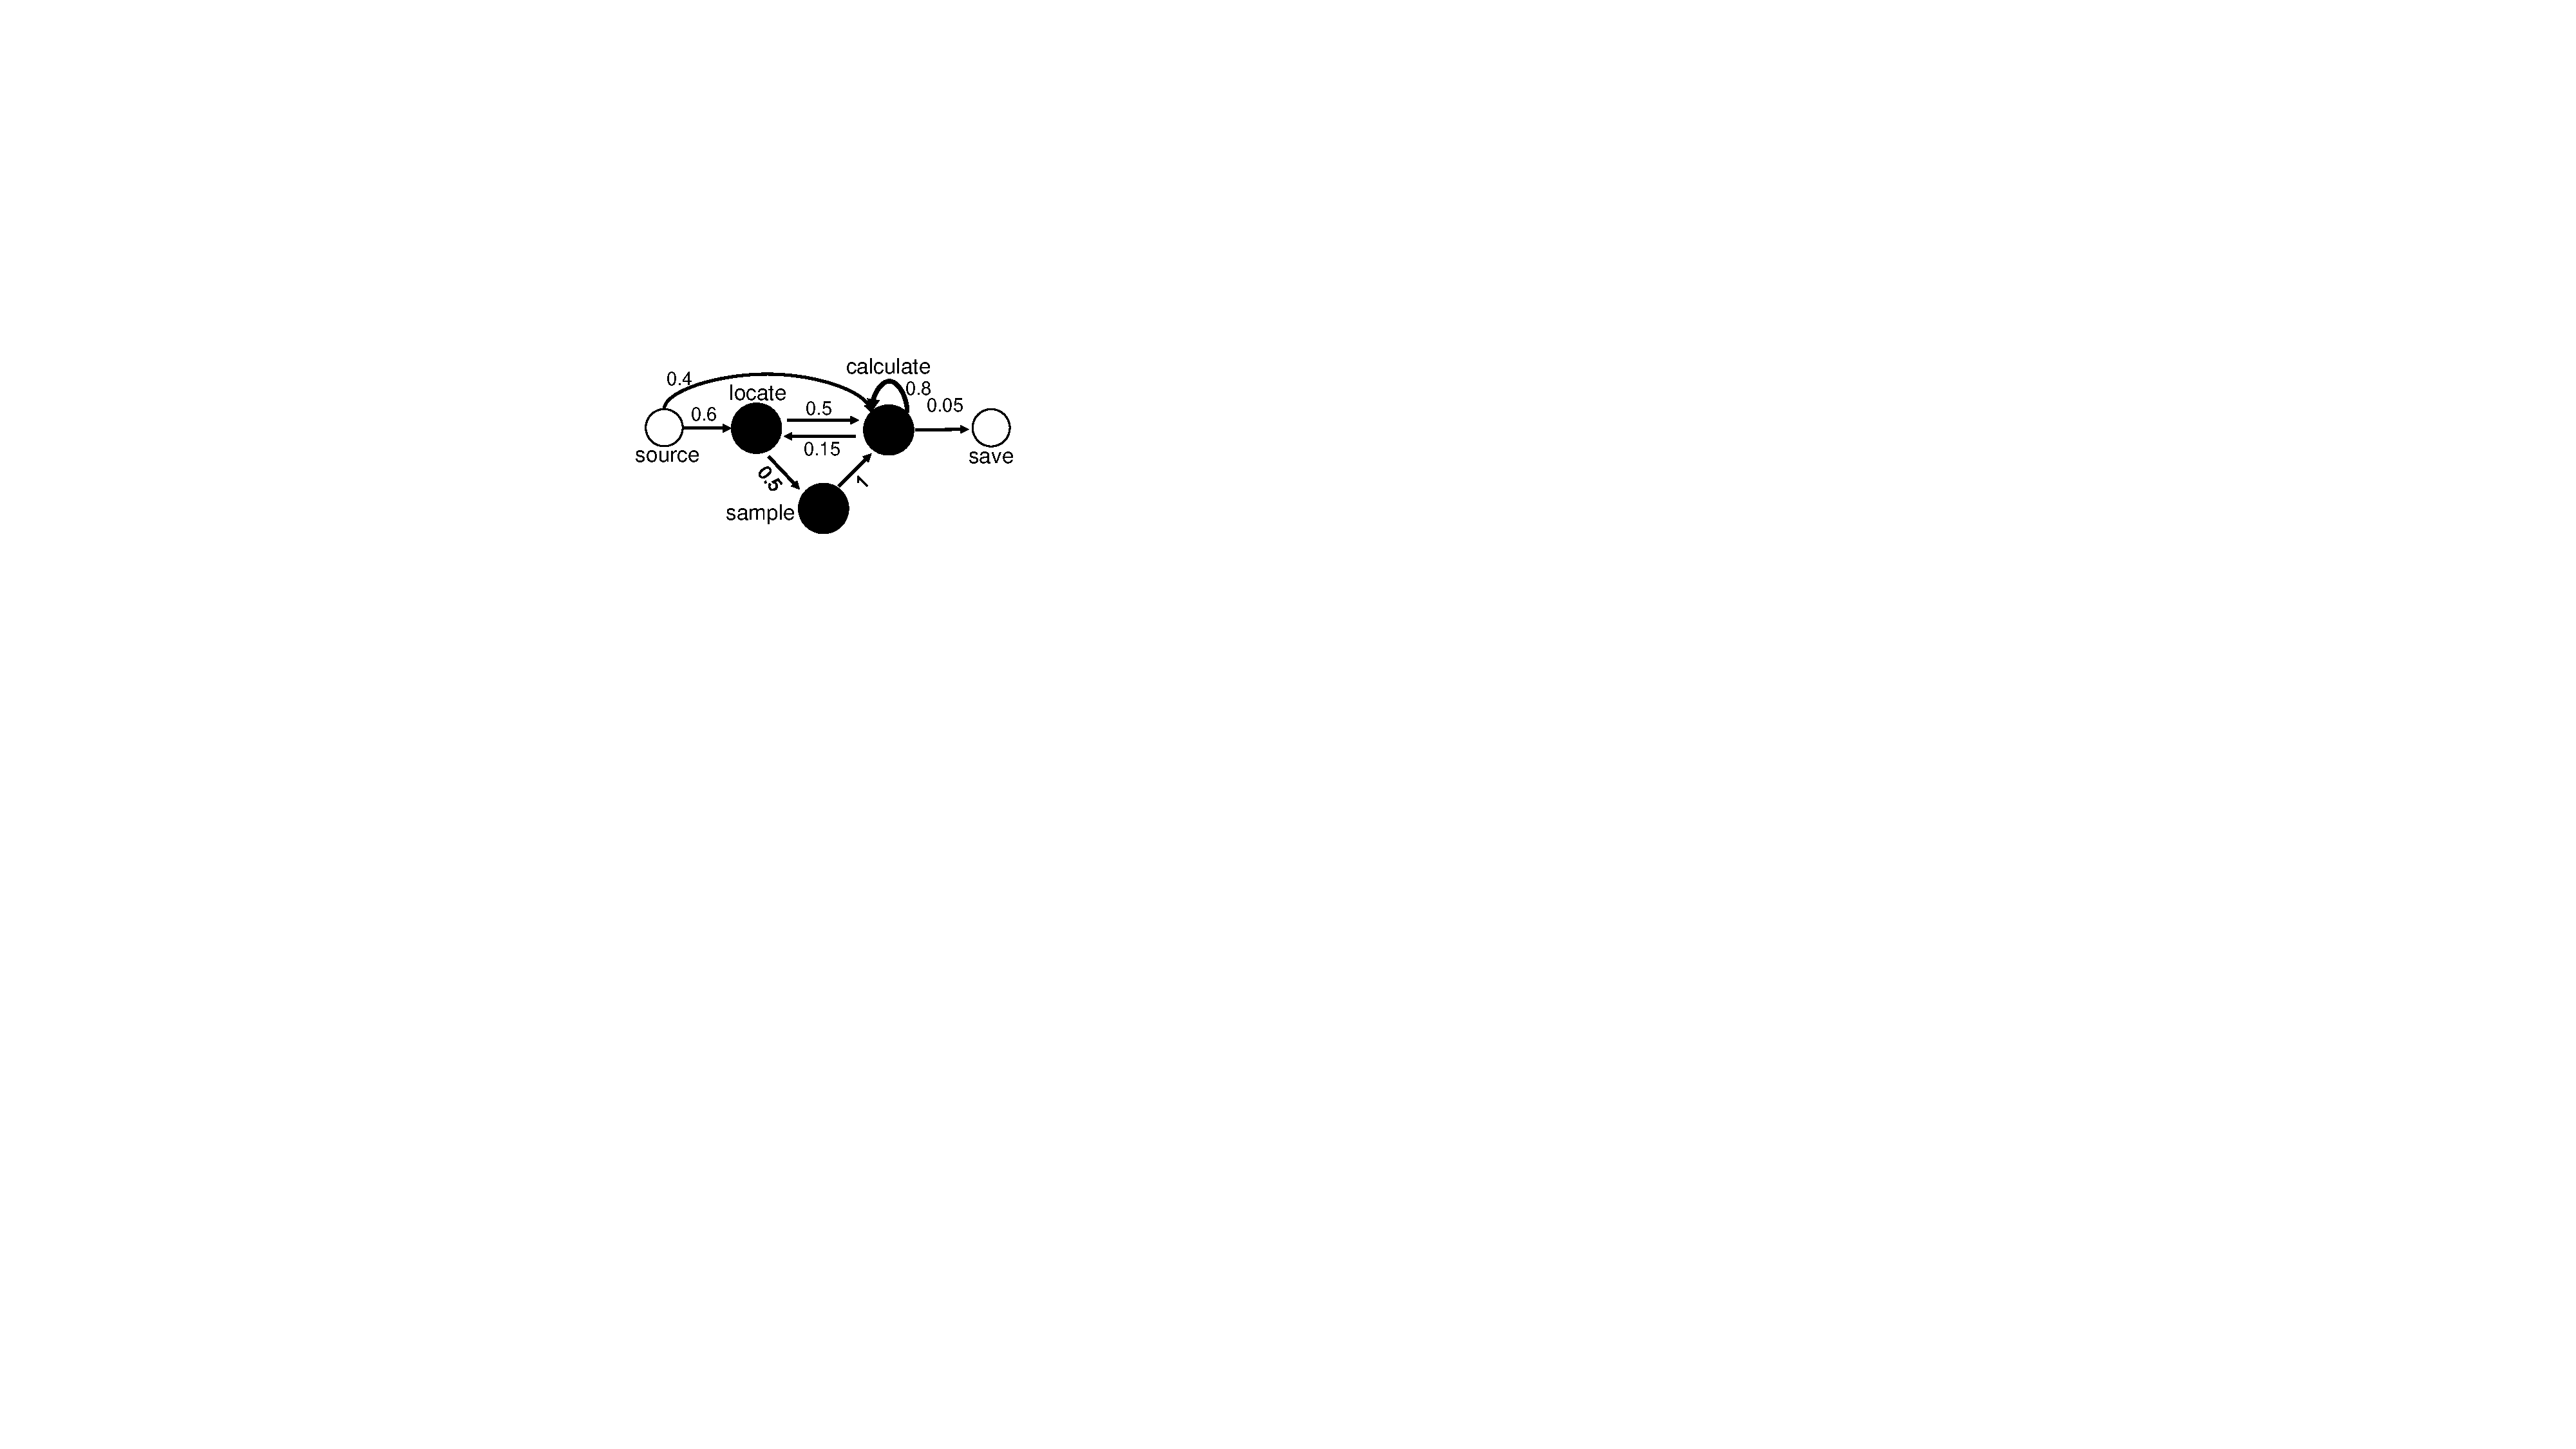
\includegraphics[width=0.5\linewidth]{figures/ml-fsm.pdf}
  \caption{ML markov chain}
  \label{fig:ml-markov}
\end{figure}

% 画图,拿机器学习 workflow 举例说明都有哪些状态,转移的关系
% 然后说,每个FSM 输出的是pipeline形状的,再使用枢纽运算符链接多个pipeline合成不同形状、大小的DAG

For the latter problem, we borrow the approach in [TDGen, Data Farm]:
It first prunes the search space using the rules in [], then for the rest physical plan, 
it specifies the data source and different workloads (mostly small workload) and runs them on all platforms to select the labels.
The platform performance on heavy workload is generated by interpolation[].
At last, we repeate the above steps on variational clusters to capture the influence on hardwares.

We trained our GCN model using the above synthesized training data.
The AUC curve is shown in Figure xx.
It can be seen that, the average training accuracy reaches around 87\%, which is acceptable enough.
What's more, the training curve of using embedding is obviously better than the one-hot.